\newpage
\section{Materiales y métodos}

Con todas las herramientas y materiales  que se exponen a continuación se ha realizado el  estudio. Se ha seguido el flujo de trabajo que se muestra en la imagen siguiente:

\begin{center}
 
    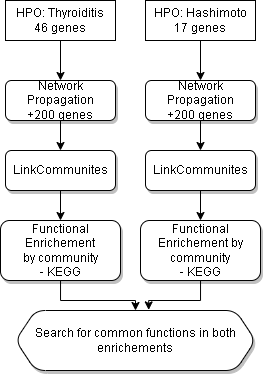
\includegraphics[scale=0.5]{figures/Diagrama sin título.drawio.png}
    
    Figure 2.1. Flujo de trabajo
\end{center}


\subsection*{Datos fenotipos}
El paso inicial fue descargar los datos genotípicos sobre los dos fenotipos a estudiar (HP:0100646 Thyroiditis y HP:0000872 Hashimoto) de la página web HPO (https://hpo.jax.org/app/).  HPO (The Human Phenotype Ontology) es un proyecto que ofrece la ontología de distintos tipos de fenotipos relevantes. Sus funciones son muy variadas; yendo desde su utilidad para dar diagnósticos médicos hasta para el uso de análisis bioinformáticos, como es el caso.
El conjunto inicial de interacciones gen-gen asociados a dichos fenotipos ha sido  obtenido a partir de la base de datos STRING (https://string-db.org/). La base de datos STRING integra conocimiento sobre las relaciones entre proteínas y genes, incluyendo desde interacciones físicas hasta relaciones funcionales. Las relaciones son determinadas a partir de una serie de evidencias con una significancia asociada. \cite{Szklarczyk2021}  Las evidencias que han determinado las redes de interacción de nuestros fenotipos son las siguientes: (1) textmining, (2) experimentos, (3) bases de datos, (4) co-expresión, (5) vecindad, (6) fusión de genes, (7) co-ocurrencia. La significancia mínima asociada a cada interacción determinada ha sido de 0.7. Finalmente, hemos encontrado un total de 46 genes asociados al fenotipo  HP: 0100646 (Thyroiditis) y 17 a  HP:0000872 (Hashimoto). 

\subsection*{Propagación de red}
Se realizó una propagación de red a los conjuntos de genes inciales (uno por cada fenotipo); obteniendo un total de 200 genes por conjunto (tal y como recomienda la literatura).\cite{Ghiassian2015} Para ello hemos usado la herramienta 'DIAMOnD' (DIseAse MOdule Detection). Esta herramienta identifica módulos que comparten 	
patrones de conectividad con el fin de determinar la principal propiedad topológica que los define, para su posterior extensión. \cite{Ghiassian2015} Se basa en algoritmos de deteccion de comunidades. Para dicha detección son usados tres métodos:
    \begin{itemize}
        \item Algoritmos de link community. Basados en similitudes de enlace entre los nodos. \cite{Ahn2010}
        \item Louvain method. Maximiza la funcion de modularidad global.\cite{Sanyal2006} 
        \item Markov Cluster Algorithm (MCL). Detecta regiones densas bansandose en un flujo aleatorio. \cite{MCL}
    \end{itemize}

Una vez detectadas todas las comunidades, éstas son evaluadas seleccionándose aquellas con una signifancia relevante (aquellas con un pvalor menor de 0.05 en el test de Fisher) \cite{Jafari2018}. El procedimiento sería el siguiente:
    \begin{itemize}
        \item La significancia de conectividad es determinada para todas los genes conectados a alguno de las comunidades detectadas.
        \item Los genes son clasificados en función de sus p-valores.
        \item Los genes con el menos p-valor se añaden a la semilla de nodos.
        \item Los pasos 1-3 se repiten añadiendo genes a las comunidades de uno en uno.
    \end{itemize}

\subsection*{LinkCommunities}
Se efectuó una búsqueda de  las comunidades presentes en ambas redes. Para dicha búsqueda usamos el paquete R 'linkcomm V1.0-11'. Linkcomm provee un conjunto de herramientas para generar, visualizar y analizar link communities en redes de tamaño y tipo arbitrario.  \cite{Kalinka2011} Se basa en un algoritmo que agrupa  los enlaces entre nodos en lugar de  agrupar los propios nodos.Esto permite que cada nodo pertenezca a múltiples comunidades, superpuestas o anidadas. \cite{Kalinka2011} 
\\
Uno de los parámetros a tener en cuenta es el threshold, el cual hace referencia a la altura a la que el dendograma es cortado. En función de este umbral, se obtienen mayor o menor número de clusters. Para este proyecto hemos optado por un threshold de 400, el cual no es demasiado restrictivo.



\subsection*{Enriquecimiento funcional}
El enriquecimiento funcional es crucial en la interpretación de datos ómicos. Este fue realizado, mediante análisis de sobrerrepresentación, a las comunidades presentes en las redes asociadas a cada fenotipo. El análisis de sobrerrepresentación es útil para determinar las funciones moleculares asociadas a un conjunto de genes. Este se encarga de determinar los procesos sobrerrepresentados (enriquecidos) dentro de un conjunto de genes mediante el test hipergeométrico. Analiza cada término KEGG, de forma aislada sin tener en cuenta la estructura de la jerarquía de términos. \cite{Zhang2010}

\\
Para su implementación se usó el paquete de R 'clusterProfiler 3.16'. Clusterprofiler fue diseñado para realizar análisis de sobrerepresentación usando términos GO y KEGG, entre otros. Actualmente soporta varias ontologías y anotaciones de pathways, y tiene miles de especies con capacidad de anotación. 
\\
Seleccionamos la ontología 'KEGG latest release 104', que  hace referencia a la Kyoto Enciclopedia de Genes y Genomas, una de las bases de datos biológicas más importantes actualmente. El mayor componente de información se denomina PATHWAY y consiste en diagramas asociados a rutas moleculares, incluyendo rutas metabólicas y regulativas. 
Se asignó a cada comunidad el pathway biólogico correspondiente en base al gene ratio obtenido tras el enriquecimiento.  El umbral del p-value ha sido fijado  en 0.05 para seleccionar solo aquellas comunidades más fieles a las distribución, tal y como se recomienda en la literatura.\cite{Jafari2018} \\  A la hora de filtrar aquellos pathways más significativos, se seleccionó también como umbral un gene ratio mayor o igual a 0.7. Para este filtrado solo tuvimos en cuenta el gene ratio de Tiroiditis.El de Hashimoto interesa que se bajo pues lo que se busca es aumentar la red de genes de dicho fenotipo.
 

